\documentclass[conference,letterpaper]{IEEEtran}
\usepackage{amsmath}
\usepackage{amssymb}
\usepackage{tikz}
\usetikzlibrary{positioning, shapes.geometric}
\usepackage{pgfplots}
\pgfplotsset{compat=1.18}

\begin{document}

    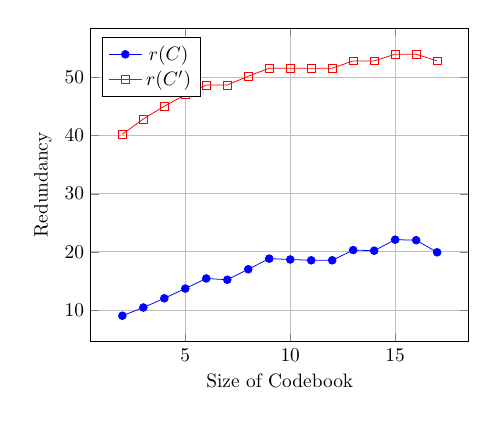
\begin{tikzpicture}[scale=0.7]
  \begin{axis}[
    xlabel={Size of Codebook},
    ylabel={Redundancy},
    grid=major,
    legend pos=north west,
  ]

  \addplot[mark=*,blue] coordinates {
    (2, 9)
    (3, 10.4150375)
    (4, 12)
    (5, 13.67807191)
    (6, 15.4150375)
    (7, 15.19264508)
    (8, 17)
    (9, 18.830075)
    (10, 18.67807191)
    (11, 18.54056838)
    (12, 18.54056838)
    (13, 20.29956028)
    (14, 20.19264508)
    (15, 22.0931094)
    (16, 22)
    (17, 19.91253716)
  };
  \addlegendentry{$r(C)$}

  \addplot[mark=square,red] coordinates {
     (2, 40.21928095)
    (3,  42.84962501)
    (4,  45.07354922)
    (5, 47)
    (6, 48.69925001)
    (7, 48.69925001)
    (8, 50.21928095)
    (9, 51.59431619)
    (10, 51.59431619)
    (11, 51.59431619)
    (12, 51.59431619)
    (13, 52.84962501)
    (14, 52.84962501)
    (15, 54.00439718)
    (16, 54.00439718)
    (17, 52.84962501)
  }; 
  \addlegendentry{$r(C')$}

  \end{axis}
\end{tikzpicture}

\end{document}